\begin{parag}{Evaluation}
	\begin{itemize}
		\item Final exam: 80\% of the grade
		\item Past year's exams are available on Moodle
		\item Two graded project milestones
			\begin{itemize}
			    \item Coding exercices build up as a small team project
			    \item Teams of 3 students: Register the teams by March 22nd
				\item Two milestones (tentative: end of Week 8 and end of Week 13)
				\item Each is wroth 10\% of the final grade
			\end{itemize}
	\end{itemize}
	
    
\end{parag}


\section{Machine Learning Basics}
\begin{parag}{What is Machine Learning}
    Machine learing takes the same form as how a human would learn, by \important{experience}. The goal is to give our \important{algorithm}, \important{data} which would output \important{insight} about our data.
\end{parag}
\begin{parag}{What data?}
    Data can be many things, it can be patient information related to births, movie reviews speech (audio file)...\\
	$ $\\
	An important thing to highlight is the difference between a \important{data set} and a \important{data sample}.
	\begin{definition}
	Data sample (or example, or point): is an individual observation
	\end{definition}
	It can be an image, a list of attributes for one patient, etc...
	\begin{definition}
	Data set: is a collection of multiple data samples. 
	\end{definition}
	Which can be a collection of images, the attributes lists for multiple patients.
\end{parag}
\begin{parag}{What insight?}
    As said before, the goal of machine learning is to output \important{insight} about our data. This is insight can be pretty much anything, the category depicted by an image, the influences between different musical genres.\\
	In this course, we will mostly focus on precise insights. In particular, we will study two classes of machine learning problems:
	\begin{itemize}
		\item Regression
		\item Classification
	\end{itemize}
\end{parag}
\subsubsection{Regression vs Classification}%

	\important{Regression} predicts \important{continuous value(s)}\footnote{As said right after, it is not continuous in the sens of a function $f$ in $ \mathbb{R}$. But value have an ordering which allows us to have an ordered set of those elements. It's just how I kind of see it} for a given sample.\\
	This means that our 'guesses' typically follow an \important{order}. We can then measure "how accurate" our prediction is: predicting 3002g instead of 2977 is better than predicting 2500g.
	On the other hand, \important{classification} use 'classes' as prediction, categories do not follow an order: predicting 'tree' instead of 'cat' is just as wrong as predicting 'car'.

	\begin{framedremark}
	
		We could first see it as in probability/statistic. Regression is the continuous case and classification is the discrete case. Although this makes 'sense', as we will see in the next remark, regression \important{doesn't mean continuous}.\\
		$ $\\
		$ $\\
	You are given a dataset of images of paintings. For each painting, you would like to predict the year it was created. Is this a regression or a classification task?\\
	It is a regression task, guessing by one year is better than being off by a complete decade.
	\end{framedremark}


\subsection{Unsupervised Learning}
\begin{parag}{Unsupervised Data}
	\begin{definition}
		In Unsupervised learning, each sample consists only of an observation, e.g., an image (without information about its content)
	\end{definition}
\end{parag}

\begin{parag}{What classes of algorithm?}
    For each learning there will be different classes of algorithms, in this case (unsupervised), the learning relies on unsupervised data. The goal is rather to analyse the observed data set.\\
	What we mean by this is that instead of trying to have direct information about our data (guess the animal on an image), we will more care about how does the data is divided etc... (splitting creating a graph of music genres)

	\begin{center}
		\href{https://www.naftaliharris.com/blog/visualizing-k-means-clustering/}{naftaliharris.com}
	\end{center}
\end{parag}
\begin{parag}{Learning Stage}
    Learning in this case consists of only one stage: Analyse the whole data, or transform it for further analysis. As said before the goal is not to make 'guesses'. Butto gives more  information about our data in order to have better insight.
\end{parag}


\chapter{Supervised Machine Learning}

\begin{parag}{Supervised Data}
    \begin{definition}
    Each sample comes with additional annotations. e.g., category label
    \end{definition}
	An assumption about the data that we are given is that the annotations (supervisory signal) are the insight that we seek to obtain from the data.\\
	This is what we are more 'used to' when it comes to machine learning. 

\end{parag}
\begin{parag}{Learning Stages}
	This times the learning is divided into two stages:
	\begin{enumerate}
		\item \textbf{Training}: Use data with ground-truth labels to optimize model parameters (see \href{http://playground.tensorflow.org}{playground.tensorflow.org})
		\item \textbf{Testing}: Predict the ouput for a new data sample
	\end{enumerate}
	
\begin{center}
\begin{tikzpicture}[
    node distance=2.1cm,
    every node/.style={font=\small},
    box/.style={
        rectangle,
        draw,
        thick,
        minimum width=3.5cm,
        minimum height=1.5cm,
        align=center
    },
    arrow/.style={
        thick,
        -{Latex[length=3mm]}
    }
]

% Nodes
\node[box] (input) {Test Image};
\node[box, right=of input] (model) {Model \\ \footnotesize (Fixed Parameters)};
\node[box, right=of model] (output) {Predicted Label};

% Arrows
\draw[arrow] (input) -- (model);
\draw[arrow] (model) -- (output);

\end{tikzpicture}
\end{center}
Here we \important{don't} use our testing data to update the model parameters. We want to check wether or not our model \important{generalizes} to the new test data which might not be the case. If we go back to the example digit guessing demo; when we try to draw a number in a corner of the box, the model is not able to correctly predict. The reason for this is that the data that our model trained on had numbers only in the middle of the box \textrightarrow not trained to other cases.
	
    
\end{parag}
\begin{parag}{Training set vs Test set}
    \begin{center}
        The training set and the test set should \important{always} be completely separate
    \end{center}

	\begin{subparag}{Remark}
	    Using the observations (inputs) is occasionally possible and referred to as transductive learning (we will not do it in this course).
	\end{subparag}
	Furthermore, we also need that our training and test samples are drawn from the \important{same statistical distribution}
    
\end{parag}

\section{Linear Model}
Let's us start with a simple supervised learning model, the goal is to start with this as our first building block and then add layer onto it (non-linearity, etc.).



\begin{parag}{Notation}
    \begin{definition}
    We denote the $i^{th}$ \important{data sample} (input) in the collection of $N$ samples as 
	\begin{align*} x_i \in \mathbb{R}^{d} \end{align*}
	a column vector of dimension $D$
    \end{definition}
	\begin{definition}
	We denote the $i^{th}$ label (output) in the collection of $N$ samples as 
	\begin{align*} y_i \end{align*}
	\end{definition}
	For \important{classification}, $y_i$ represents the category the samples belongs to. Whereas for \important{regression}, $y_i$ can be a single continuous value, or a column vector of dimension $C$.
\end{parag}


\begin{parag}{Example}
	\begin{itemize}
		\item In the following toy example, $x_i$ is one 2D point, and thus $D = 2$
		\item $y_i$ is a discrete value indicating the class (color), i.e., 1, 2, or 3
	\end{itemize}
	\begin{center}
	
\includegraphics[scale=0.3]{screenshots/2026-02-20.png}
	\end{center}
	As another example, we can take the digit recognition example, $x_i$ is a grayscale image. If it has height $H$ and width $W$, then $D =  H \cdot  W$.
	\begin{center}
	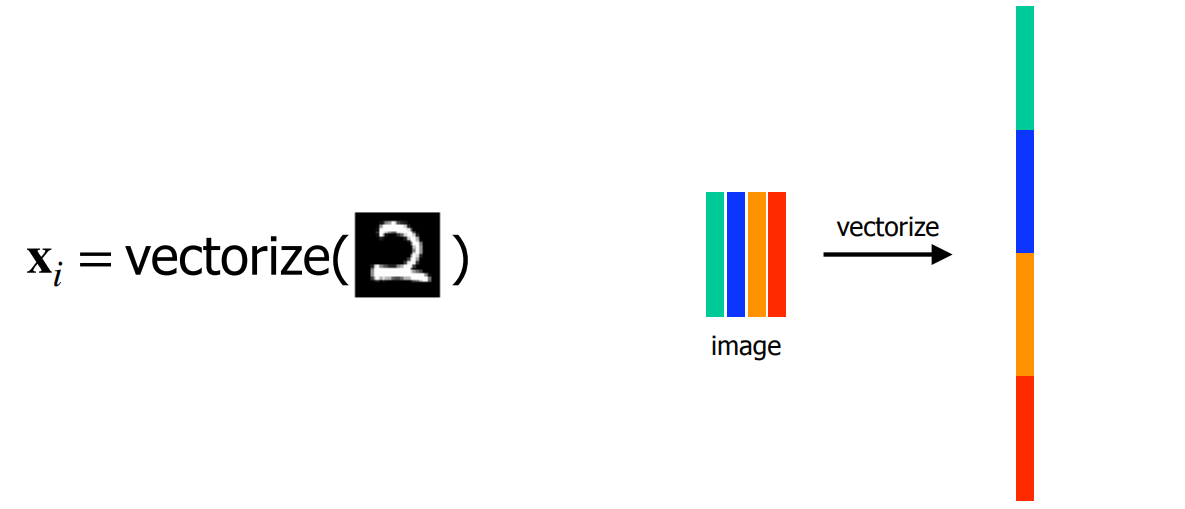
\includegraphics[scale=0.3]{screenshots/2026-02-20_1.png}
	\end{center}
	What we are essentially doing is transforming our image (which is a matrix in our case) to a vector by mapping each element of this message to a 'row' of the vector (this is the same a when we store a matrix in a row-major way).\\

	In this case of digit recognition, the output $y_i$ is a single discrete value indicating the digit, e.g. $y_i = 2$
\end{parag}


\begin{parag}{Our first machine learning model}
    To start things off, let us create the \important{simplest} model possible:
	\begin{itemize}
		\item A single input dimension, $D = 1$
		\item A single output dimension, $C = 1$
	\end{itemize}
	Our goal is to solve a regression task (the output is continuous). We seek to predict the weight of a fish given its length:

\end{parag}
	
\begin{center}
\begin{tikzpicture}[
    node distance=3.0cm,
    every node/.style={font=\small},
    box/.style={
        rectangle,
        draw,
        thick,
        minimum width=3.5cm,
        minimum height=1.5cm,
        align=center
    },
    arrow/.style={
        thick,
        -{Latex[length=3mm]}
    }
]

% Nodes
\node (input) {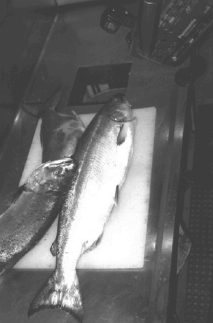
\includegraphics[scale=0.2]{screenshots/2026-02-20_2.png}};
\node[box, right=of input] (model) {Length};
\node[box, right=of model] (output) {Weight};

% Arrows
\draw[arrow] (input) -- (model);
\draw[arrow] (model) -- (output);
\node[above left=0.08cm of model, align=center] (test) {Some computer \\  vision algorithm};
\node[above right= 0.08cm of model, align=center](test2) {Our machine \\ learning algorithm};

\node[below=1cm of model] (inputDim) {1D input ($D =  1$)};
\node[below=1cm of output] (outputDim) {1D ouput ($C =  1$)};

\draw[arrow, dashed] (inputDim) -- (model);
\draw[arrow, dashed] (outputDim) -- (output);

\end{tikzpicture}
\end{center}
	
\begin{parag}{ $ $}
    Given $N$ annotated data samples $\left\{\left(x_i, y_i\right)\right\}$ with (length, weight) measurements, we can plot the data ($N =  8$ here):
	\begin{center}
	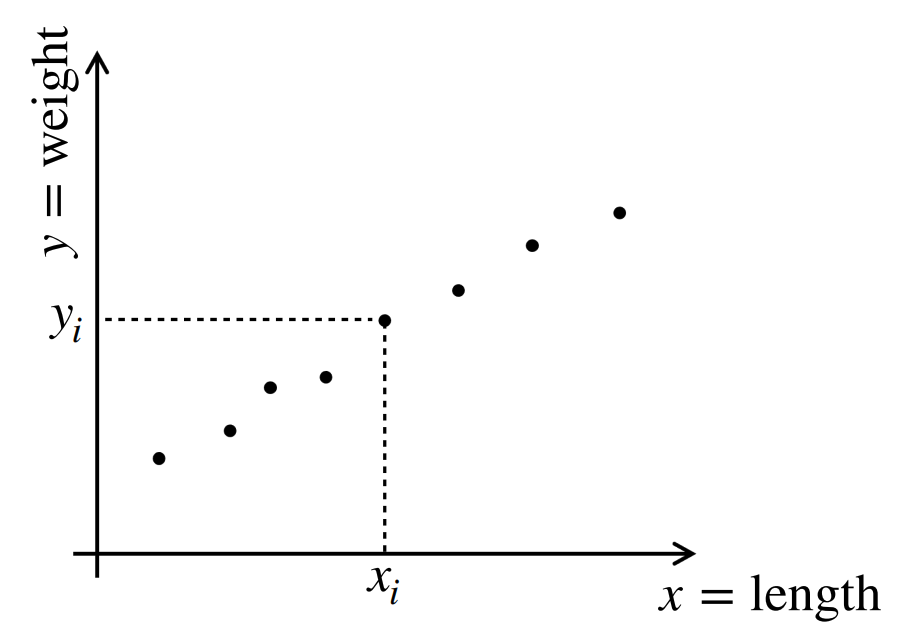
\includegraphics[scale=0.25]{screenshots/2026-02-20_3.png}
	\end{center}
	We can see here that there is a kind of trend going on in this data set, we seek to approximate it with a line:
	\begin{center}
	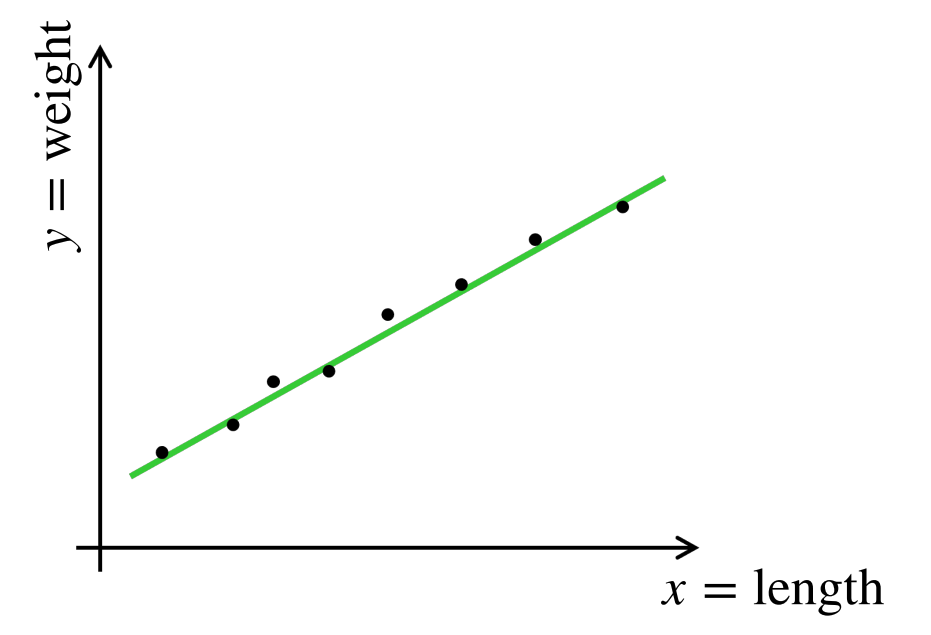
\includegraphics[scale=0.25]{screenshots/2026-02-20_4.png}
	\end{center}
	Once we have defined the line based on the $N$ training samples, we can use it to predict the weight of any new length (again, assuming the test data follows the same distribution as the training data).
\end{parag}

\begin{parag}{A simple parametric model: The line}
    Now let us think a bit more about the model, what is it made of? To be able to define a line we need 2 parameters:
	\begin{itemize}
		\item the $y$-intercept, we will call it $\omega^{\left(0\right)}$
		\item The slope $\omega^{\left(1\right)} = \frac{\Delta y}{\Delta x}$
	\end{itemize}
	With this two parameters, we can express any line 
	\begin{align*} y = \omega^{\left(0\right)}  + \omega^{\left(1\right)}x\end{align*}
	This relation above \important{is} our model.
\end{parag}
\begin{parag}{Line fitting}
    Now that we have our model, let us acutally fit our model to some data. Given $N$ pairs $\left\{\left(x_i, y_i\right)\right\}$, the goal is to find the line that passes through these observations. But is this possible? Not really there is always noise in our data. The goal of fitting here is to find the line that \important{best fits} this observation and if you remember linear algebra, we actually have some tools to do so.
\end{parag}



\begin{parag}{1D Linear Regression training}
	In essence, fitting a line consists of finding the best line parameters $\omega^{\left(0\right)\ast}$ and $\omega^{\left(1\right)\ast}$ for some given data. This corresponds to the training stage:
	\begin{itemize}
		\item Given $N$ training pairs $\left\{\left(x_i, y_i\right)\right\}$, we aime to find $\left(\omega^{\left(0\right)}, \omega^{\left(1\right)}\right)$, such that the predictions of the model 
			\begin{align*} \hat{y}_i = \omega^{\left(0\right)} + \omega^{\left(1\right)}x_i \end{align*}
			are close to the true values $y_i$
	\end{itemize}
	We then need to define a measure of closeness, or conversely an error, between $y_i$ and $\hat{y}_i$.
	
	As seen in linear algebra, a natural measure of the error is the Euclidean distance (also called $L_2$ norm)
	\begin{align*} d(\hat{y}_i, y_i) = \sqrt{\left(\hat{y}_i - y_i\right)^2} \end{align*}
	\begin{center}
	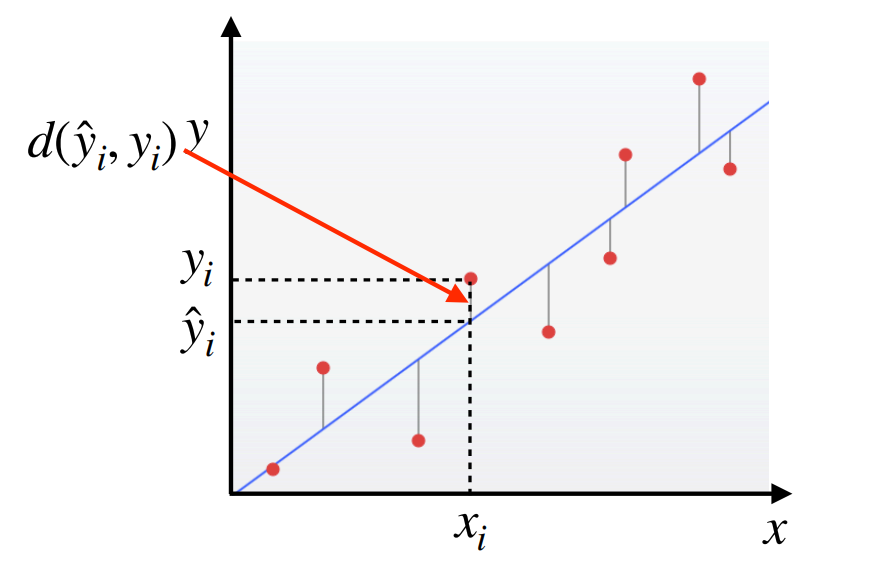
\includegraphics[scale=0.25]{screenshots/2026-02-20_5.png}
	\end{center}
	In practice, one prefers to use the square of this distance:
	\begin{align*} d^2\left(\hat{y}_i, y_i\right) = \left(\hat{y}_i - y_i\right)^2 \end{align*}
	With this definition, traning can be translated as a least-square problem minimization problem:
	\begin{align*} \left(\omega^{\left(0\right)\ast}, \omega^{\left(1\right)\ast}\right) =  \text{argmin}_{\omega^{\left(0\right)}, \omega^{\left(1\right)}} \frac{1}{N}\sum_{i = 1}^{N}d^2\left(\hat{y}_i, y_i\right) \end{align*}
	Where $\hat{y}_i$ depends on $\omega^{\left(0\right)}$ and $\omega^{\left(1\right)}$
	A nicer way which will be useful when using multi-dimension model, is to write our model as a matrix $W$ such that 
	\begin{align*} \hat{y}_i = W x_i  \end{align*}
	\begin{align*} x_i \in \mathbb{R}^2 \end{align*}
	In our case as we have $y$ being a one dimensional vector, we don't have to write our $W$ as a matrix, a vector is sufficient:
	\begin{align*} x_i =  \begin{pmatrix} 1 \\ x_i \end{pmatrix} \in \mathbb{R}^2 \mathspace \mathspace \mathspace w = \begin{pmatrix} w^{\left(0\right)} \\ w^{\left(1\right)} \end{pmatrix} \in \mathbb{R}^2 \end{align*}
	Which gives us:
	\begin{align*} 
		R\left(w\right) = \frac{1}{N}\sum_{i = 1}^{N}\left(w^{T}x_i - y_i\right)^2 = \frac{1}{N}\sum_{i= 1}^{N}\left(x_i^Tw - y_i\right)^2
	\end{align*}
	As said above, in general, an input observation $x_i$ is not represneted by a single value. If we take a grayscale image, it can be represented by an $ W\cdot H$ dimensional vector
	\begin{align*} x_i \in \mathbb{R}^{28 \cdot  28} = \mathbb{R}^{784} \end{align*}
\end{parag}

